%% Meghan Sullivan
%% 20171205
%% Bifactor model with two specific factors; north south

% standalone class for individual image to be included in a document
% border=15pt controls the whitespace padding around the diagram
\documentclass[border=15pt]{standalone}

% load custom style configurations from separate file
%% ------------------------------------------------------------
%% Charlie Redmon
%% 20170923
%% semTikzStyle.tex: style configurations for SEM path diagrams
%% ------------------------------------------------------------

\usepackage{tikz}

% observed variable
\tikzstyle{ov}=[shape=rectangle,
                draw=black!80,
                minimum height=0.6cm,
                minimum width=0.6cm,
                thick]

% response variable
\tikzstyle{av}=[shape=rectangle,
                draw=black!80,
                fill=black!10,
                minimum height=0.6cm,
                minimum width=0.6cm,
                thick]

% latent variable
\tikzstyle{lv}=[shape=circle,
                draw=black!80,
                thick,
                minimum width=1cm]

% correlations
\tikzstyle{lcor}=[bend left=30, dashed]
\tikzstyle{rcor}=[bend right=30, dashed]

% self-loops (for variance)
\tikzstyle{lloop}=[loop left, 
                   out=210, 
                   in=150, 
                   distance=0.3cm,
                   densely dotted]

\tikzstyle{rloop}=[loop right, 
                   out=30, 
                   in=-30, 
                   distance=0.3cm,
                   densely dotted]

\tikzstyle{aloop}=[loop above, 
                   out=60, 
                   in=120, 
                   distance=0.3cm,
                   densely dotted]

\tikzstyle{bloop}=[loop below, 
                   out=-60, 
                   in=-120, 
                   distance=0.3cm,
                   densely dotted]




\begin{document}

%% ">=stealth" sets the arrow head style
%% "semithick" sets the line width (0.6 pt)
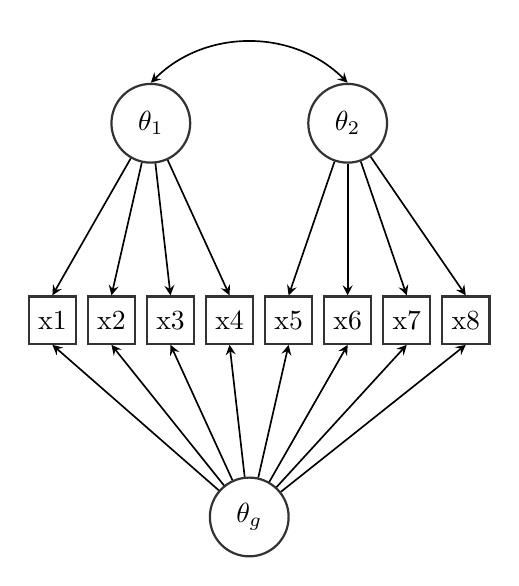
\begin{tikzpicture}[>=stealth,semithick,scale=0.5]

% observed variables
\node[ov] (y1) at (-10,0)     {x1};
\node[ov] (y2) at (-8.5,0)  {x2};
\node[ov] (y3) at (-7,0)  {x3};
\node[ov] (y4) at (-5.5,0)  {x4};
\node[ov] (y5) at (-4,0)  {x5};
\node[ov] (y6) at (-2.5,0)    {x6};
\node[ov] (y7) at (-1,0)  {x7};
\node[ov] (y8) at (0.5,0)  {x8};

% latent variables
\node[lv] (f1) at (-7.5, 5)  {$\theta_1$};
\node[lv] (f2) at (-2.5, 5)  {$\theta_2$};
\node[lv] (f3) at (-5, -5)  {$\theta_g$};

% paths
\path[->] (f1) edge node[above=0.08cm,scale=0.8,pos=0.7] {} (y1.north);
\path[->] (f1) edge node[above=0.08cm,scale=0.8,pos=0.7] {} (y2.north);
\path[->] (f1) edge node[above=0.08cm,scale=0.8,pos=0.7] {} (y3.north);
\path[->] (f1) edge node[above=0.08cm,scale=0.8,pos=0.7] {} (y4.north);
\path[->] (f2) edge node[above=0.08cm,scale=0.8,pos=0.7] {} (y5.north);
\path[->] (f2) edge node[above=0.08cm,scale=0.8,pos=0.7] {} (y6.north);
\path[->] (f2) edge node[above=0.08cm,scale=0.8,pos=0.7] {} (y7.north);
\path[->] (f2) edge node[above=0.08cm,scale=0.8,pos=0.7] {} (y8.north);

\path[->] (f3) edge node[above=0.08cm,scale=0.8,pos=0.9] {} (y1.south);
\path[->] (f3) edge node[above=0.08cm,scale=0.8,pos=0.9] {} (y2.south);
\path[->] (f3) edge node[above=0.08cm,scale=0.8,pos=0.9] {} (y3.south);
\path[->] (f3) edge node[above=0.08cm,scale=0.8,pos=0.9] {} (y4.south);
\path[->] (f3) edge node[above=0.08cm,scale=0.8,pos=0.9] {} (y5.south);
\path[->] (f3) edge node[above=0.08cm,scale=0.8,pos=0.9] {} (y6.south);
\path[->] (f3) edge node[above=0.08cm,scale=0.8,pos=0.9] {} (y7.south);
\path[->] (f3) edge node[above=0.08cm,scale=0.8,pos=0.9] {} (y8.south);

\path[<->] (f1.north) edge [bend left=45] node[left,scale=0.8] {} (f2.north);

\end{tikzpicture}



\end{document}
